In questo capitolo vengono spiegati nel dettaglio la struttura e il funzionamento del backend di scansione adottato dal progetto.

\section{Storia del progetto}
\textbf{OpenVAS} (\emph{Open Vulnerability Assessment Scanner}) è una piattaforma \emph{open source} per la rilevazione, l'analisi e la gestione di vulnerabilità e falle di sicurezza.

OpenVAS Nasce nel 2005 come \emph{fork} dello scanner \textbf{Nessus}, quando questi modificò la propria licenza, diventando da \emph{open source} un software proprietario distribuito sotto licenza commerciale. La comunità open source da quel momento ha manutenuto il fork risultante, inizialmente denominato \emph{GNessUs} e poi rinominato in \emph{OpenVAS}. Tempo dopo entrò a far parte dei progetti supportati economicamente dalla \emph{Software in the Public Interest}.

Tra i principali contributori del fork vi erano gli sviluppatori di Intevation e DN-Systems, aziende che poi sarebbero diventate Greenbone AG e finanziate dalla BSI tedesca (l'Ufficio Federale per la Sicurezza Informatica). Eventualmente nel 2008 la neo-costituita Greenbone si propose tra gli obiettivi aziendali il sostenere lo sviluppo open source di OpenVAS e creare delle versioni maggiormente supportate e curate per i clienti enterprise, oltre all'offrire il necessario supporto. Oltre a Greenbone, con il tempo si unirono al progetto altre aziende per contribuire eventualmente ad un feed stabile e aggiornato di test di vulnerabilità, componente chiave ed essenziale dell'intero progetto.

Eventualmente già nel 2010 OpenVAS ruppe la compatibilità con Nessus e negli anni successivi ricevette ulteriore supporto dalla BSI e anche dalla DFN (la rete di ricerca tedesca usata da università e centri di ricerca), nella forma di avvisi di sicurezza regolari pubblicati sotto licenza GPL.

Nel 2017 i contributi di Greenbone diventarono palesi con un cambio di nome ufficiale: il progetto non si sarebbe più chiamato \emph{OpenVAS framework}, ma \textbf{Greenbone Vulnerability Management (GVM)}, un framework completo di sicurezza informatica, dove per OpenVAS si intende solo lo scanner vero e proprio, uno dei tanti componenti.

\section{Modello di business}
Greenbone OpenVAS e GVM possono ricevere gli aggiornamenti di sicurezza e configurazioni da due feed, entrambi manutenuti da Greenbone:
\label{feed}
\begin{itemize}
    \item \textbf{Greenbone Community Feed}: questo canale di aggiornamenti è totalmente gratuito e open-source. Contiene versioni minimali e preconfigurate di configurazioni di scansione, liste di porte, reportistica; ma soprattutto, in questo feed non sono incluse tutti i test di vulnerabilità disponibili, limitandosi a fornire esclusivamente quelli più critici e importanti. I dati sono aggiornati giornalmente secondo una policy di best effort e senza garanzie di alcun tipo.
    \item \textbf{Greenbone Enterprise Feed}: questo canale di aggiornamenti è invece a pagamento, ed è pensato per i clienti di Greenbone che usano il framework GVM in contesti aziendali. In questo canale sono forniti tutti i test di vulnerabilità disponibili, ma anche tutte le configurazioni di scansione e reportistica. Il servizio è inoltre garantito sotto SLA\footnote{\emph{Service Level Agreement}: contratto in cui un provider di un servizio garantisce agli utenti di quel servizio degli standard minimi di qualità e disponibilità.}
\end{itemize}
Il progetto è sostenuto economicamente soprattutto attraverso la sottoscrizione al secondo feed da parte dei clienti di tipo \emph{enterprise}. In aggiunta, Greenbone fornisce anche \emph{hardware appliance}\footnote{Dispositivi fisici progettati per eseguire una specifica funzione / applicazione, ottimizzati espressamente per quell'unico scopo.}, \emph{virtual appliance}\footnote{Sistemi informatici virtuali che eseguono una specifica funzione / applicazione, progettati per essere installati e usati in un software di virtualizzazione.} e una soluzione SaaS gestita direttamente da loro.

\subsection{Greenbone Operating System (GOS)}
Questo sistema operativo è quello che anima le \emph{appliance} fornite da Greenbone. Di fatto è poco più di un insieme di \emph{wrapper} grafici, TUI\footnote{Terminal User Interface} e non, per facilitare la manutenzione del sistema. Il software integra anche il supporto commerciale di Greenbone e vari miglioramenti di esperienza utente.

\section{Architettura}
L'architettura del framework Greenbone Vulnerability Management (GVM) è costituita da numerosi componenti interconnessi.

\subsection{gvmd}
Il demone UNIX \texttt{gvmd} è il cuore del framework GVM. Esso ha compiti di gestione e interconnessione tra tutte le principali componenti di basso livello del sistema, offrendo un'API di gestione operabile con il protocollo \textbf{Greenbone Management Protocol (GMP)}.

In particolare:
\begin{itemize}
    \item Comunica con lo scanner OpenVAS vero e proprio tramite il protocollo \textbf{Open Scanner Protocol (OSP)}.
    \item Legge e scrive sul database (di \emph{default} un'istanza di PostgreSQL) i dati ricevuti dai feed configurati, i risultati delle scansioni e il sistema di utenti e ruoli interno al framework GVM.
    \item Fa da server per \textbf{GSA}, l'interfaccia web nativa e ufficiale di Greenbone, di fatto la modalità naturale usata per amministrare l'intero sistema.
\end{itemize}

Si noti che il demone può anche essere operato direttamente senza passare per \textbf{GSA}. Questo è possibile sempre tramite l'API offerta sotto protocollo GMP, consentendo quindi di creare strumenti personalizzati di automazione, ma anche vere e proprie interfacce alternative.

\begin{figure}
    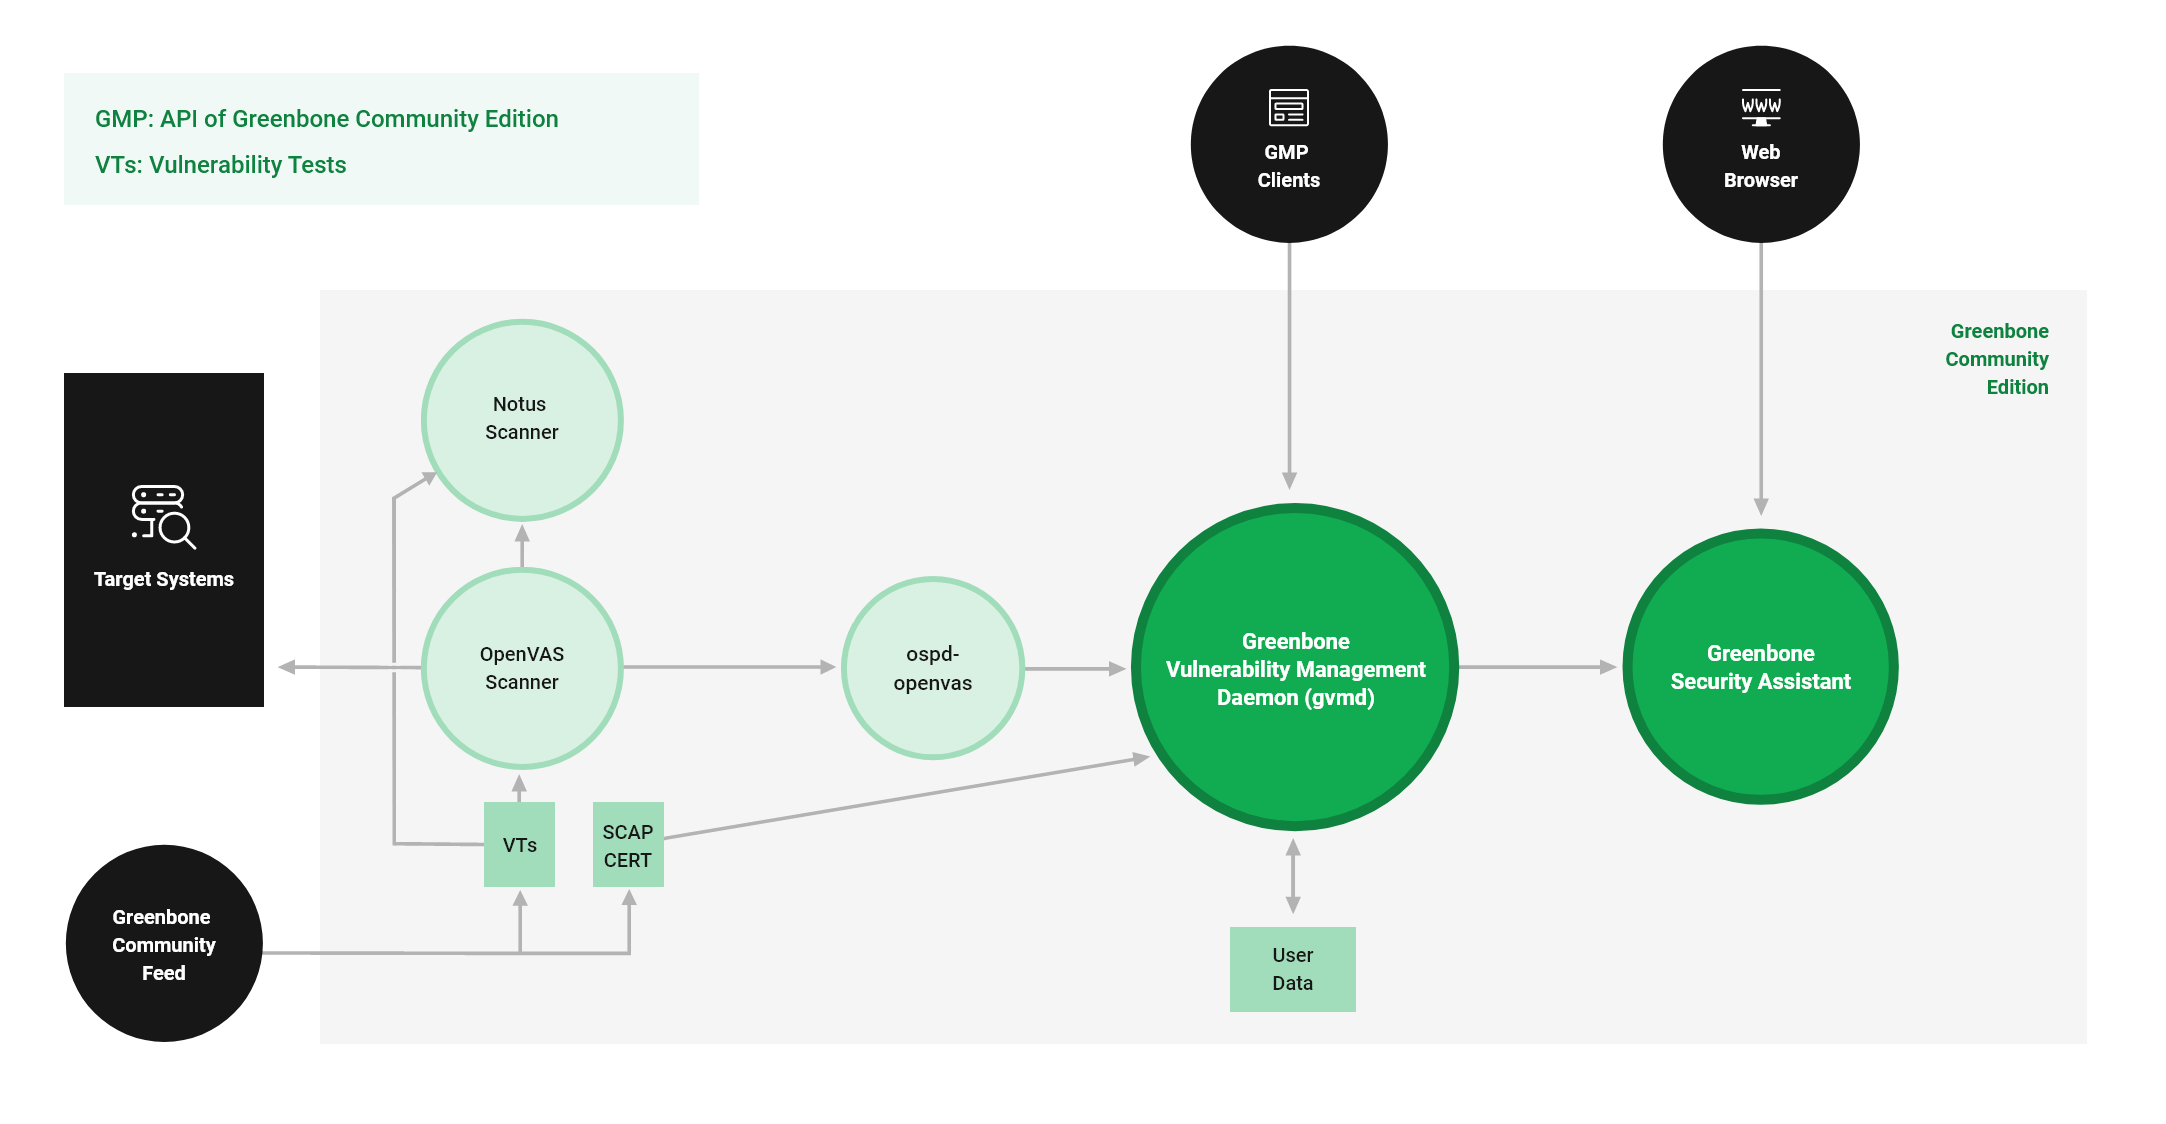
\includegraphics[width=\textwidth]{img/greenbone-community-22.4-architecture.png}
    \caption{Architettura della release 22.4}
\end{figure}

\subsection{GSA}
\textbf{Greenone Security Assistant (GSA)}, ovvero l'interfaccia web nativa di Greenbone (realizzata con React), pensata per l'interazione umana / da parte dell'utente finale attraverso browser.

\subsubsection{gsad}
Si tratta del web server che offre GSA. Di fatto svolge anche le funzioni di backend (che invece fa le veci del semplice frontend). Realizzato interamente in C standard.

\subsection{VT}
Gli scanner veri e propri eseguono delle ``applicazioni'' sui sistemi bersaglio per trovare le vulnerabilità. Questi programmi sono i cosiddetti \textbf{Vulnerability Test (VT)} anche detti talvolta \textbf{Network Vulnerability Test (NVT)}. Essi sono scritti nel linguaggio \textbf{NASL}.

\subsubsection{Linguaggio NASL}
\textbf{NASL (NASL Attack Scripting Language)} è un \emph{Domain Specific Language} interpretato, con lo scopo di definire test per rilevare vulnerabilità su dispositivi di rete. Offre funzioni integrate di supporto per facilitare questo tipo di codifica.

Gli script NASL vengono normalmente eseguiti all'interno delle scansioni OpenVAS, ma possono anche essere eseguiti direttamente dall'utente tramite l'interprete NASL fornito (\texttt{openvas-nasl}).

\subsection{SCAP (CVE, CPE)}
\textbf{SCAP (Security Content Automation Protocol)} è uno standard aperto creato nei primi anni del 2000 dal \textbf{NIST}\footnote{National Institute of Standard and Technology} statunitense, uno dei principali riferimenti attualmente in termini di cybersecurity. Scopo dello standard SCAP è regolare i processi organizzativi di valutazione della sicurezza delle risorse informatiche e quindi automatizzarli.

A tal fine, SCAP comprende un insieme di standard, definiti \textbf{componenti}. Segue una lista dei principali:
\begin{itemize}
    \item \textbf{Common Vulnerabilities and Exposures (CVE)}: fornisce e assegna identificativi univoci alle vulnerabilità note.
    \item \textbf{Common Platform Enumeration (CPE)}: standardizza la descrizione dell'inventario informatico (applicazioni, servizi software, sistemi operativi, hardware) sin nei minimi dettagli.
    \item \textbf{Common Configuration Enumeration (CCE)}: identifica univocamente diverse configurazioni di sistema.
    \item \textbf{Common Vulnerability Scoring System (CVSS)}: valuta la severità di una vulnerabilità attraverso un punteggio $\in [0,10]$.
\end{itemize}

In GVM è integrato un servizio che attraverso i feed menzionati in \ref{feed} aggiorna continuativamente i dati SCAP di cui ha bisogno. In particolare, vengono sfruttati i dati \textbf{CVE} e \textbf{CPE}.

Il framework inoltre mette a disposizione tramite \textbf{GSA} un calcolatore del punteggio \textbf{CVSS}.

\subsection{OpenVAS e Notus}
Lo scanner incluso nel sistema è ovviamente \textbf{OpenVAS}, ma esiste anche un altro ``scanner'' utilizzabile, \textbf{Notus}. Questo in realtà non è nient'altro che un componente Python che razionalizza e ottimizza la verifica degli script NASL.

\subsubsection{openvasd}
Si noti tuttavia che a partire dalla versione 23.0 di OpenVAS è stato introdotto \texttt{openvasd}: questo nell'intenzione di Greenbone vuole essere un unico demone che integra al suo interno tutte le funzioni di OpenVAS (lo scanner vero e proprio), Notus (l'ottimizzazione degli script NASL) e \texttt{ospd-openvas} (l'intermediario che usa il protocollo \textbf{OSP} per mediare la comunicazione tra scanner e \texttt{gvmd}). Il demone sarà riscritto con il linguaggio Rust, per renderlo più performante e moderno, risultando in una migliore manutenibilità. Inoltre, l'API OSP sarà sostituita da una API HTTP.

\section{Installazione}
Laddove l'edizione Enterprise è solitamente fornita nelle \emph{appliance}, rendendo di fatto inutile l'installazione, l'edizione gratuita invece deve essere installata dall'utente e configurata secondo le sue esigenze.

Di fatto, esistono due modi in cui il sistema può essere installato e quindi gestito:
\begin{itemize}
    \item \textbf{Compilato da sorgenti}: l'utente deve scaricare il codice sorgente dalle \emph{repository} pubbliche e compilarlo manualmente.
    
    Questo procedimento ovviamente non è consigliato in produzione, visto il rischio di instabilità.
    \item \textbf{Greenbone Community Containers}: in questo formato i singoli componenti precedentemente discussi sono segregati in \emph{container} Docker, garantendo riproducibilità di versioni e funzionalità. Tramite \texttt{docker-compose} i container sono quindi orchestrati e gestiti secondo l'architettura precedentemente esposta.
\end{itemize}

Numerose distribuzioni Linux offrono anche dei pacchetti precompilati nelle loro \emph{repository} native, ma Greenbone ufficialmente non offre supporto per eventuali errori derivanti dall'installazione e dall'uso seguente di queste edizioni, non essendo coinvolta nel processo di compilazione impiegato.

\section{Motivazioni alla base della scelta}
I principali motivi alla base di questa scelta sono:
\begin{itemize}
    \item \textbf{Disponibilità di una versione gratuita}: OpenVAS può essere installato e amministrato direttamente dall'azienda senza costi di licenze o abbonamenti, preoccupandosi solo di predisporre e manutenere l'hardware necessario.
    
    Tuttavia, è importante far notare ancora una volta come la versione gratuita di OpenVAS non disponga di tutti i test di sicurezza disponibili, rendendo necessaria un'ulteriore analisi per verificare se i dati forniti siano sufficienti agli scopi aziendali.

    \item \textbf{Open source}: OpenVAS è open source, perciò il suo codice è liberamente visibile se necessario, evitando durante lo sviluppo il rischio di incorrere in componenti non documentati o comunque opachi.
    
    \item \textbf{Librerie ufficiali}: inoltre, Greenbone mantiene anche degli strumenti ufficiali per interfacciarsi con il sistema OpenVAS, tra cui soprattutto una libreria Python che cerca di implementare quante più funzionalità del protocollo GMP.
\end{itemize}